Legato provides an S\+MS Inbox service to allow apps to receive S\+MS messages through their own, private message box, without\+:


\begin{DoxyItemize}
\item Having to manage S\+IM or modem memory;
\item Conflicting with other applications that also receive S\+MS messages;
\item Missing messages while being updated or restarted.
\end{DoxyItemize}

The S\+MS Inbox Service handles the resource arbitration for the user app\+: the message reception is always guaranteed, for example the user app doesn\textquotesingle{}t have to worry about freeing space in the S\+IM (or device\textquotesingle{}s storage area) when it is full.

In fact, at device\textquotesingle{}s startup or when a S\+IM is inserted, the S\+IM content is copied into the \char`\"{}\+Inbox
   Message Storage\char`\"{} folder allocated in the root file system of the device. Then, the process frees automatically the S\+IM content. Moreover, every new received S\+MS message is automatically copied into the \char`\"{}\+Inbox
   Message Storage\char`\"{} folder and deleted from the S\+IM. This mechanism keeps the S\+IM always empty in order to guarantee the reception of S\+MS messages.

This process is the same when the S\+MS message storage is the device\textquotesingle{}s storage area (ME -\/ Mobile Equipment).

The message box is a persistent storage area. All files are saved in the directory /mnt/flash/sms\+Inbox.There are two directories named \char`\"{}cfg\char`\"{} and \char`\"{}msg\char`\"{}. \char`\"{}cfg\char`\"{} directory contain two json files\+: le\+\_\+sms\+Inbox1.\+json \& le\+\_\+sms\+Inbox2.\+json which contains msg\+Ids of messages. \char`\"{}msg\char`\"{} directory contains json files named $<$message\+\_\+no$>$.json. It contains message information like \char`\"{}imsi,\char`\"{}format\char`\"{},\char`\"{}text\char`\"{},\char`\"{}pdu\char`\"{},\char`\"{}msg\+Len" etc.

The creation of S\+MS inboxes is done based on the message box configuration settings (cf. \hyperlink{c_smsInbox_le_smsInbox_configdb}{Configuration tree} section). This way, the message box contents will be kept up to date automatically by the S\+MS Inbox Service, even when the user app is slow to start, is stopped while it is being updated, or is being restarted to recover from a fault.

A message box works as a circular buffer, when the message box is filled, the older messages are deleted to free space for new messages. But, the application can also explicitly delete messages if it doesn\textquotesingle{}t need them anymore.

A First \& Second message box (named le\+\_\+sms\+Inbox1 \& le\+\_\+sms\+Inbox2) can be used by application. These 2 message boxes are used independently. All functions of this second message box are prefixed by le\+\_\+sms\+Inbox2 (instead of le\+\_\+sms\+Inbox1).The user can implement other message boxes based on le\+\_\+sms\+Inbox1 and le\+\_\+sms\+Inbox2 model.

Necessary modifications for adding / removing message box\+:


\begin{DoxyItemize}
\item Modify le\+\_\+sms\+Inbox.\+c by adding / removing the message box name in le\+\_\+sms\+Inbox\+\_\+mbox\+Name\mbox{[}\mbox{]} list and define the message box wrappers using D\+E\+F\+I\+N\+E\+\_\+\+M\+B\+X() macro.
\item Customize the \char`\"{}provides api\char`\"{} section of the component.\+cdef by adding the message box name as an api.
\end{DoxyItemize}


\begin{DoxyImageNoCaption}
  \mbox{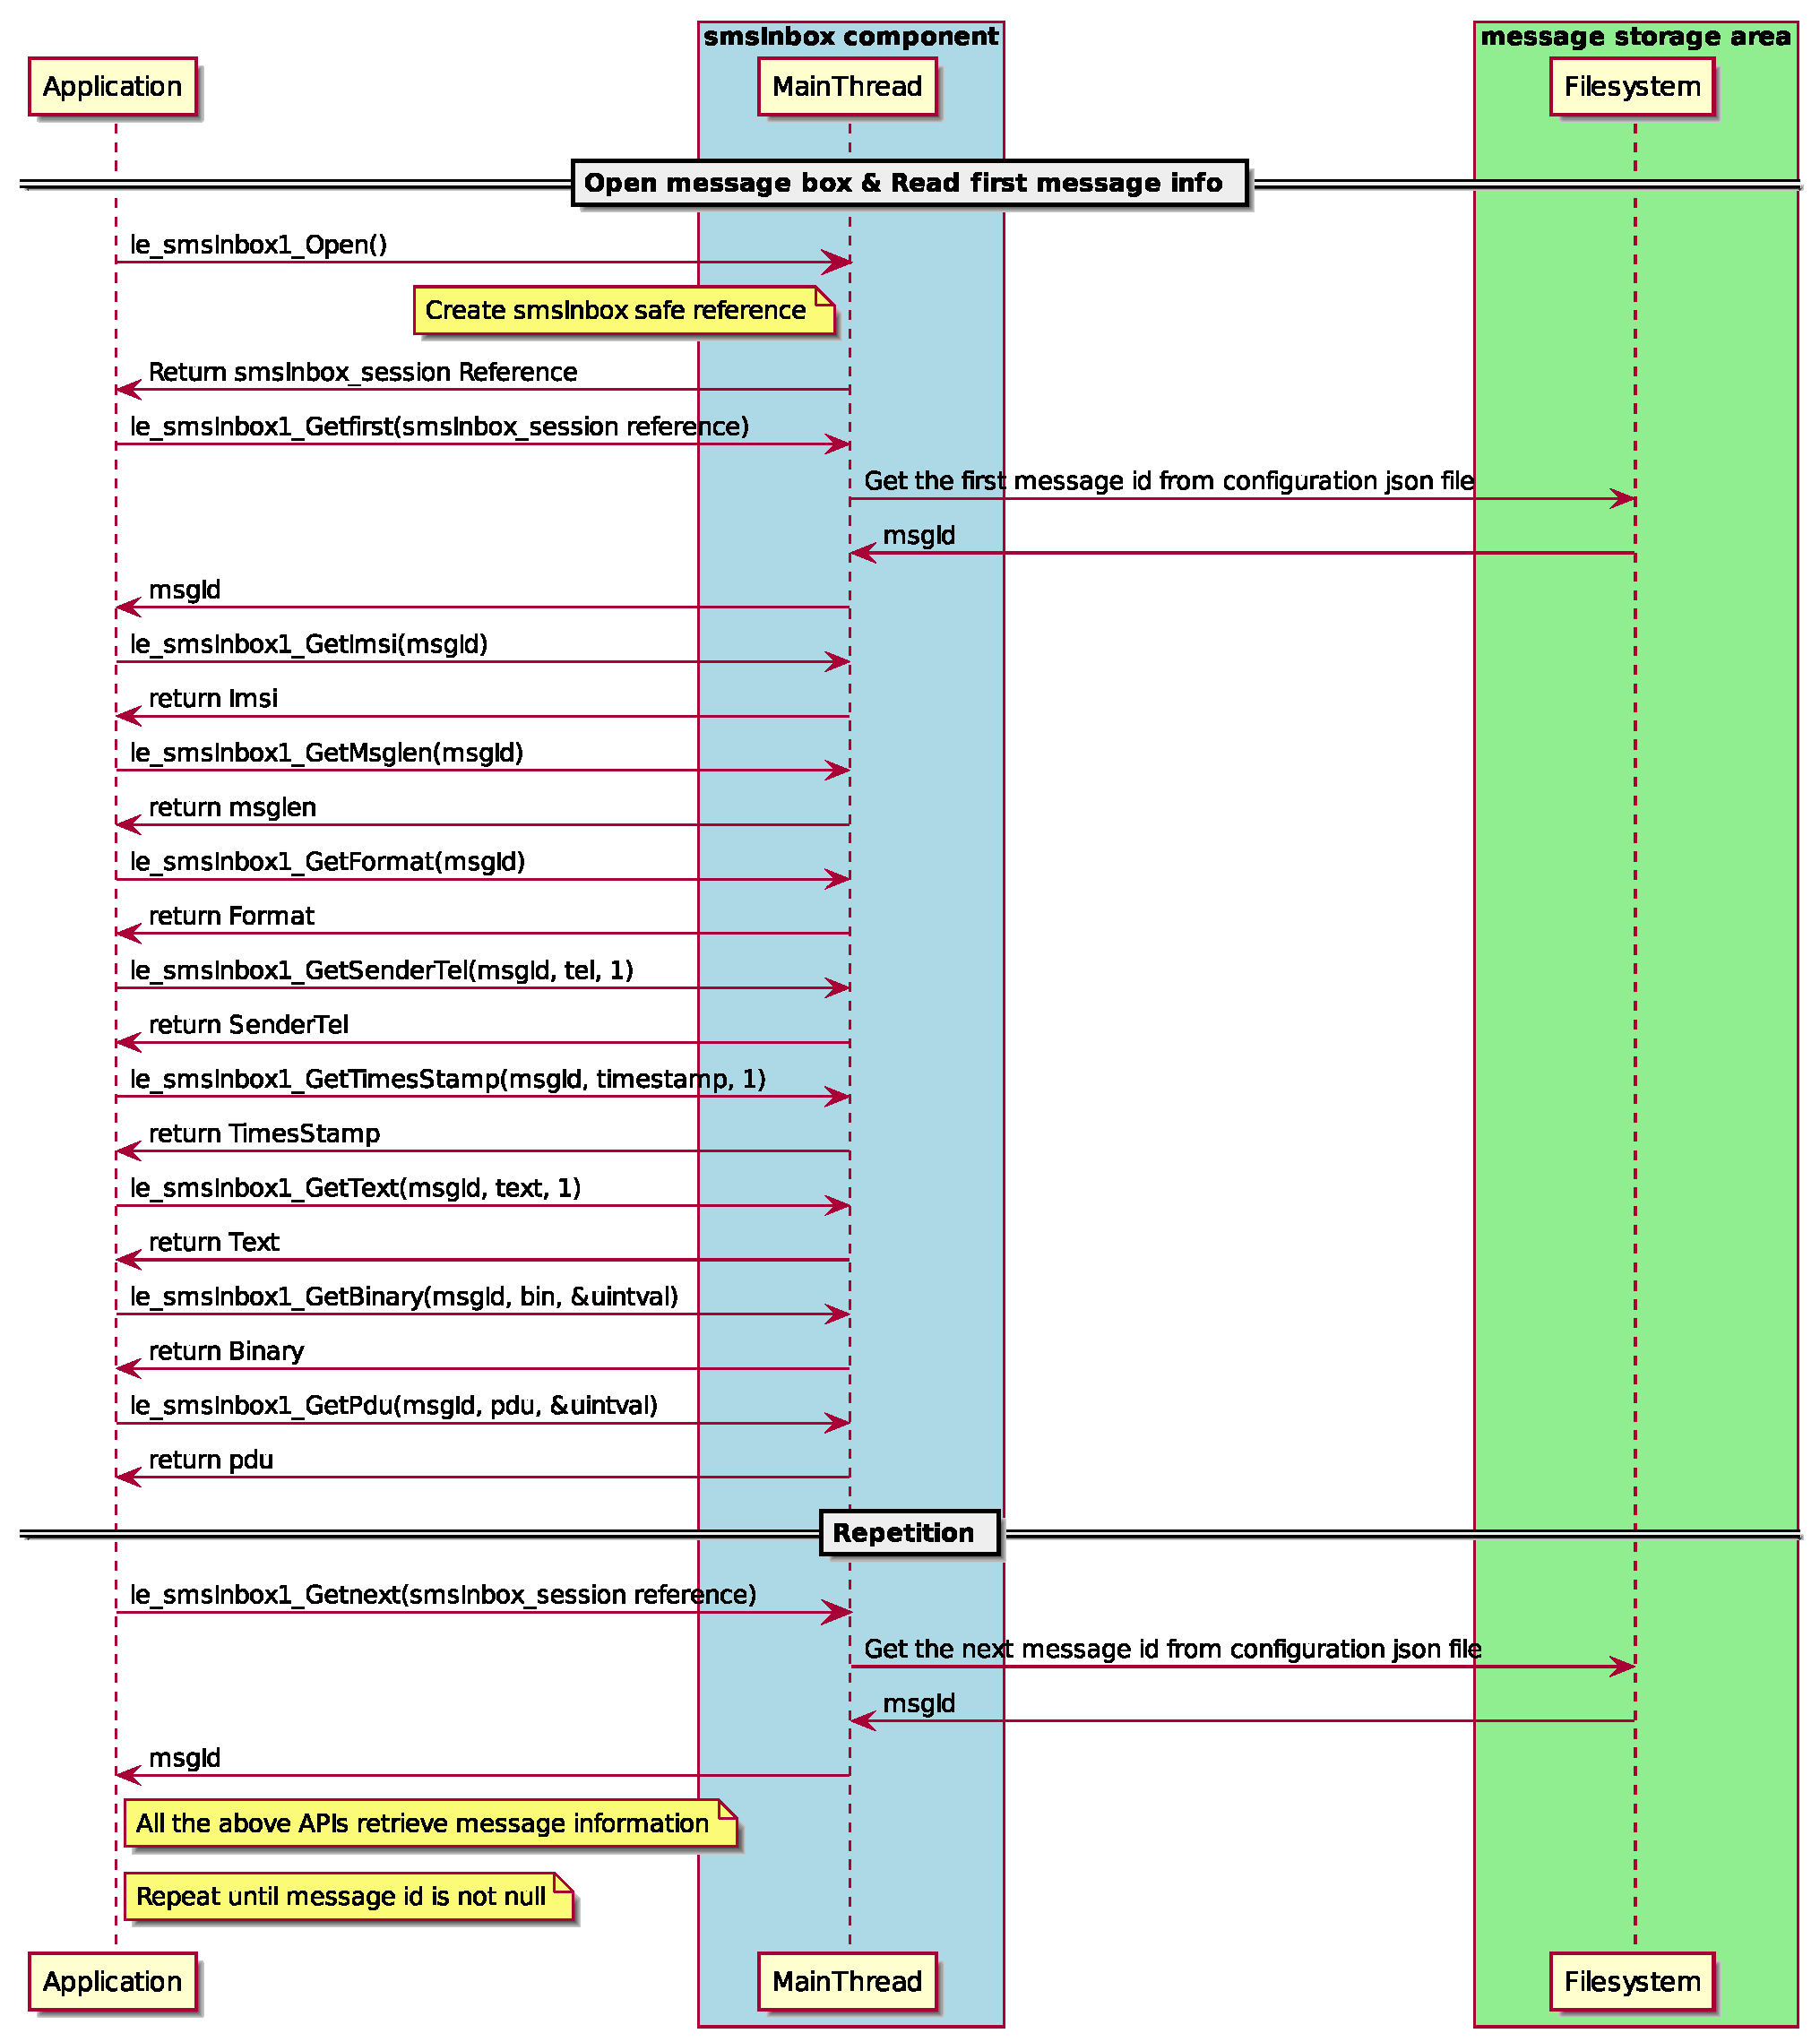
\includegraphics[width=\textwidth,height=\textheight/2,keepaspectratio=true]{le_smsInbox_GetMessage}}
\end{DoxyImageNoCaption}
 Copyright (C) Sierra Wireless Inc. 